
\documentclass{article}

\usepackage{p200}
\usepackage[colorlinks=true,linkcolor=blue]{hyperref}

\hypersetup{pdftitle = {Physics 203 } }
\hypersetup{pdfauthor = {}, pdfsubject = {Physics} }

\pagestyle{headings}

\begin{document}

\setcounter{page}{1}

\begin{tikzpicture}[remember picture,overlay]
\node [xshift=-1in,yshift=-1in] at (current page.north east) [below left] {Name: \underline{\makebox[2in]{}}};
\end{tikzpicture}

\begin{center}
\LARGE{Physics 203 Quiz 1} \\[2mm]
\small{\sf Jun 26, 2013}
\end{center}

\thispagestyle{empty}

\section*{Word Problems}
Show all your work and circle your final answer. (Ten points each.) \par


\textbf{1.} \quad When an electron and a positron (its antimatter twin) collide they
typically annihillate in a burst of electromagnetic energy. Assume all
the energy from the mass of the pair (each equal to \(9.11 \times 10^{-31}\)
kilograms) is converted into two photons of energy. What is the
wavelength of these photons?
\par {\footnotesize\sf Answer: \(2.43 \times 10^{-12}\) meters}
\par The total mass involved is twice the value given in the problem---one
for each particle. Thus,
%
\begin{equation*}
m = (2)(\sci{9.11}{-31})
= \sci{1.822}{-30}
\end{equation*}
The energy involved in this mass is given by
%
\begin{equation*}
E = mc^2
= (\sci{1.822}{-30})(\sci{3.00}{8})^2
= \sci{1.6398}{-13}
\end{equation*}
But since there are two photons, each carries \(8.199 \times 10^{-14}\) joules
of energy. Using Planck's formula, $E = hf$, the frequency must be
%
\begin{equation*}
\sci{8.199}{-14} = (\sci{6.626}{-34})(f)
\implies f = \sci{1.2356}{20}
\end{equation*}
The wavelength is given by $c = f\lambda$, so
%
\begin{equation*}
\sci{3.00}{8} = (\sci{1.2356}{20})(\lambda)
\implies \sci{2.4263}{-12}
\end{equation*}
This is in the gamma ray portion of the electromagnetic spectrum.
\newpage

\textbf{2.} \quad An evil genius wants to shrink the Moon in order to steal it. He
accidentally shrinks its below it Schwarzschild radius and the Moon
is lost forever in a mini-black hole. What is this radius?


\begin{center}
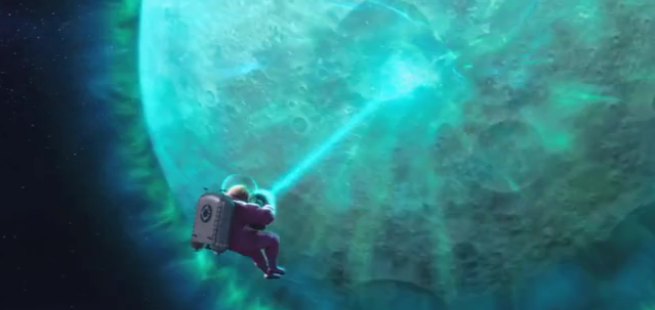
\includegraphics[scale=0.4]{C:/"Program Files"/my/github/spot/content/images/gru-shrinks-moon2.png}

\label{fig:gru-shrinks-moon2-png}
\end{center}
\par {\footnotesize\sf Answer: 0.109 millimeters}
\par We simply use the definition of the Schwarzschild radius:
%
\begin{equation*}
r_s = \frac{2GM}{c^2}
\end{equation*}
The $GM$ value for the moon is
%
\begin{equation*}
GM = (\sci{6.673}{-11})(\sci{7.36}{22})
= \sci{4.9113}{12}
\end{equation*}
So...
%
\begin{equation*}
r_s = \frac{(2)(\sci{4.9113}{12})}{(\sci{2.998}{8})^2}
= \sci{1.0929}{-4}
\end{equation*}
\newpage


\end{document}